% !TEX root = ./../../_Thesis.tex

% section's Name and Label
%\section{Absolute Threshold}
%\label{sec:AbsoluteThreshold}

In addition to the previously discussed optical aberrations that affect visual perception, there are non-optical characteristics (\ie, intrinsic individual phenomena) that could be considered in the simulation to achieve more realistic renderings of retinal images. In this section, we discuss an attempt to estimate one such intrinsic characteristic --- the {\it absolute threshold for vision} or simply {\it absolute threshold} or  
{\it minimum visible}.  
%(also known as the {\it minimum visible}) %with optical aberrations values. 
%Also, we try to integrate it in the optical simulation pipeline. 
%When an imaging system (\eg, the human eye) is mis-focused at a point in the scene, 
The light emitted/reflected by an out-of-focus scene point is spread out across some area of the observer's retinal surface, producing a so-called {\it circle of confusion} and causing blur (Figure~\ref{fig:coc}). Since the eye's photoreceptors have an energy threshold for triggering a neural signal indicating light detection, the larger the circle of confusion (and consequent spread of the incoming energy), the bigger should be the light intensity required to trigger such neural signal. Thus, considering an individual without any condition that reduces the translucency of the eye along its optical path (\eg, cataracts), we have formulated the following hypothesis: 

\vspace{0.2cm}
\noindent
{\bf H1}:
%By considering this statements, we've created the following hypothesis:
{\it The absolute threshold for vision is directly proportional to the magnitudes of the eye's defocus (\ie, myopia or hyperopia) and astigmatism.
As such, the absolute threshold can be used as an estimate of the spherical equivalent of the eye's refractive error}. 
\\

The {\it spherical equivalent} is the sum of the spherical (defocus) plus half of the cylindrical (astigmatism) values of the optical system (\ie, $S + 0.5 \times C$) expressed in diopters.

\begin{figure}[h]
	\centering
	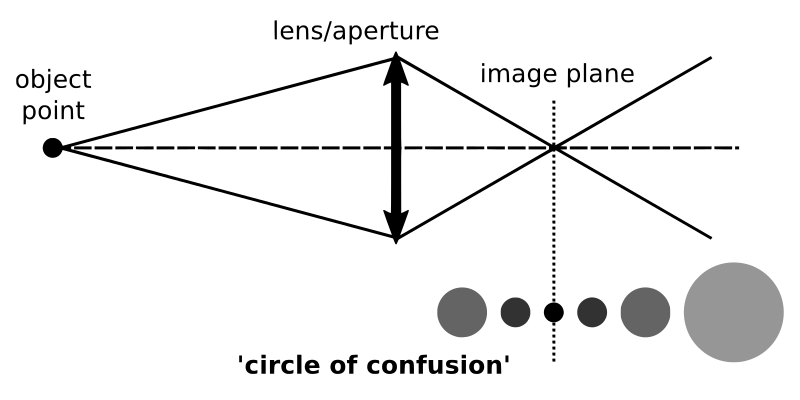
\includegraphics[width=0.6\linewidth]{__Images/04/mv_insight.png}
	\caption[Geometrical perspective of the circle of confusion]{The image of an in-focus point is formed on the image plane. An out-of-focus point, on the other hand, projects a so-called circle of confusion on the image plane, causing blur. The radius of the circle is proportional to the amount of defocus.} 
%	Geometrical perspective of the circle of confusion}
	\label{fig:coc}
\end{figure}

The following subsections discuss a psychophysical experiment established to estimate the absolute threshold information of an eye. The population sample is presented together with the quasi-random algorithm used during the experiments. 
%Finally, we detail a simple way for generating retinal images deeming this specific non-optical aberration.